\chapter{Fundamente teoretice în sisteme de recomandare}
\label{chap:ch3}

Acest capitol prezintă fundamentele teoretice care stau la baza sistemelor de recomandare, punând accent pe metodele utilizate în practică: filtrarea bazată pe conținut și filtrarea colaborativă.
De asemenea, sunt remarcate provocările cu care aceste sisteme se confruntă, precum problema „cold start”, ambiguitățile semantice și aspecte legate de securitate și confidențialitate.
Aceste concepte teoretice oferă cadrul necesar pentru înțelegerea și dezvoltarea unui sistem de potrivire între persoane.

\section{Filtrare bazată pe conținut}
\label{sec:ch3sec1}

Filtrarea bazată pe conținut este o tehnică de recomandare care analizează atributele unui element sau ale unei persoane pentru a genera sugestii.
În general, această metodă este utilizată cu scopul de a oferi recomandări personalizate în funcție de profilul utilizatorilor.
Sistemul identifică similarități între profiluri și sugerează elemente sau persoane care corespund cel mai bine preferințelor utilizatorului \cite{kumar2018recommendation}.
\par
Această metodă este des utilizată în platforme precum Spotify, YouTube sau Netflix, în special pentru a recomanda conținut similar cu cel deja consumat. 
De exemplu, un utilizator care ascultă muzică jazz va primi mai frecvent recomandări din aceeași zonă muzicală, fără a fi nevoie de comparații cu preferințele altor utilizatori. 
Avantajul major al acestui tip de filtrare constă în caracterul său personalizat, axat strict pe gusturile fiecărui utilizator, fără a fi influențat de tendințele generale ale comunității.
\par
Cu toate acestea, filtrarea bazată pe conținut are și unele limitări. 
Una dintre cele mai notabile este lipsa diversității — sistemul poate rămâne „prizonier” în tiparele stabilite inițial și poate recomanda doar conținut foarte similar cu ceea ce a fost deja consumat. 
În plus, eficiența sistemului depinde de calitatea datelor și de granularitatea atributelor folosite pentru descrierea obiectelor.

\subsection{Principiu de funcționare}
\label{subsec:ch3sec1sub1}
Metoda se bazează pe construirea unui profil pentru fiecare utilizator, care reflectă preferințele sale în funcție de conținutul anterior accesat sau evaluat. 
Acest profil este comparat cu descrierile altor elemente disponibile, iar sistemul recomandă acele elemente care prezintă cele mai mari similarități.
De regulă, se folosesc tehnici de procesare a limbajului natural, metode probabilistice sau modele de învățare automată.
Una dintre particularitățile filtrării bazate pe conținut este faptul că nu are nevoie de date despre alți utilizatori pentru a funcționa. Recomandările sunt generate exclusiv pe baza preferințelor și comportamentului.
Acest lucru oferă o flexibilitate ridicată, în special atunci când predilecțiile se schimbă. Pe de altă parte, această abordare presupune existența unor descrieri detaliate ale elementelor din sistem, ceea ce poate deveni o provocare atunci când aceste informații lipsesc sau sunt dificil de structurat \cite{ISINKAYE2015261}.
\section{Filtrare colaborativă}
\label{sec:ch3sec2}
Filtrarea colaborativă este o metodă eficientă de recomandare, care se bazează pe preferințele utilizatorilor pentru a oferi sugestii relevante.
În contrast cu filtrarea bazată pe conținut, filtrarea colaborativă utilizează date colectate din interacțiunile utilizatorilor cu scopul de a identifica puncte comune între aceștia.
Principiul presupune că persoanele cu gusturi și comportamente asemănătoare vor aprecia și recomanda elemente similare.
Există două modalități de abordare în acest tip de filtrare: filtrarea bazată pe utilizatori și filtrarea bazată pe itemi.
Prima variantă generează recomandări pe baza preferințelor altor utilizatori cu profiluri similare, în timp ce a doua variantă analizează obiectele și le identifică pe acelea care au fost evaluate pozitiv de către utilizatorii asemănători \cite{schafer2007collaborative}.

\subsection{Abordare tehnică}
\label{subsec:ch3sec2sub1}
În mod concret, filtrarea presupune construcția unei matrici utilizator-item \ref{FigUserItemMatrix}, unde rândurile reprezintă utilizatorii, iar coloanele obiectele (produse, cărți, filme etc.). 
Valorile din matrice reprezintă evaluările sau aprecierile persoanelor față de itemi. Pentru a determina similaritatea, se folosesc diferite metrici, precum Pearson, cosinus sau Jaccard.
Pe baza acestora, algoritmul determină utilizatorii cei mai apropiați și creează un grup de persoane similare denumit vecinătate \cite{kumar2018recommendation}.
\begin{figure}[htbp]
	\centering
    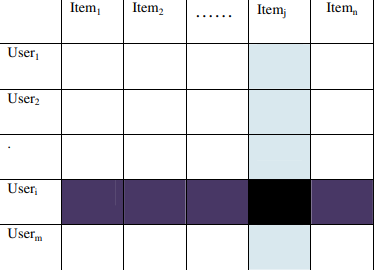
\includegraphics[scale=1]{./figures/user-item-matrix.png}
	\caption{Matrice utilizator-item \cite{ISINKAYE2015261}}
	\label{FigUserItemMatrix}
\end{figure}


\section{Metrici de similaritate}
\label{sec:ch3sec3}
Un pas esențial în oferirea unei recomandări este calculul similarități dintre utilizatori sau itemi. 
În continuare, vor fi prezentate cele mai importante metode de evaluare a asocierilor \cite{sondur2016similarity}.

\subsection{Coeficientul Jaccard}
\label{subsec:ch3sec3sub1}
Coeficientul Jaccard \cite{bag2019efficient} este o metrică folosită cu precădere la compararea seturilor. 
Este definit ca raportul între mărimea intersecției și cea a uniunii celor două seturi \ref{eq:jaccard}.
\begin{equation}
    Jaccard(A, B) = \frac{|A \cap B|}{|A \cup B|}
    \label{eq:jaccard}
\end{equation}

\subsection{Similaritatea cosinus}
\label{subsec:ch3sec3sub2}
Similaritatea cosinus \cite{al2018similarity} este metodă utilizată frecvent pentru a măsura asemănarea dintre doi vectori. 
Formula \ref{eq:cosinus} se bazează pe unghiul dintre vectorii respectivi într-un spațiu n-dimensional, unde \(A_i\), respectiv \(B_i\) reprezintă valorile vectorilor de pe poziția \(i\).
\begin{equation}
    cos(A, B) = \frac{\sum_1^n A_i \cdot B_i}{\sqrt{\sum_1^n A_i^2 \cdot \sum_1^n B_i^2}}
    \label{eq:cosinus}
\end{equation}

\subsection{Corelația Pearson}
\label{subsec:ch3sec3sub3}
Corelația Pearson \cite{al2018similarity} exprimă gradul de relație liniară dintre două variabile vectoriale, fiind utilizată pentru a evalua variația a două seturi de date.
Formula \ref{eq:Pearson} este adesea folosită pentru a compara intensități sau ratinguri, unde \(\bar{A_i}\) și \(\bar{B_i}\) reprezintă media aritmetică a valorilor vectorilor.
\begin{equation}
    Pearson(A, B) = \frac{\sum_1^n (A_i - \bar{A}) \cdot (B_i - \bar{B})}{\sqrt{\sum_1^n (A_i - \bar{A})^2 \cdot \sum_1^n (B_i - \bar{B})^2}}
    \label{eq:Pearson}
\end{equation}


\section{Provocări și limitări ale metodelor de recomandare}
\label{sec:ch3sec4}
Deși sistemele de recomandare bazate pe conținut și colaborative au un rol esențial în personalizarea experienței utilizatorilor, acestea se confruntă cu o serie de limitări care pot afecta eficiența și precizia recomandărilor. 
Printre cele mai întâlnite provocări se numără lipsa datelor suficiente pentru utilizatorii noi, dificultatea de a surprinde preferințele în schimbare și complexitatea modelării relațiilor între elemente sau utilizatori. 
În continuare sunt prezentate câteva dintre aceste probleme, împreună cu implicațiile lor asupra performanței sistemelor de recomandare.

\subsection{Problema „Cold start”}
\label{subsec:ch3sec4sub1}
Problema „Cold start” \cite{lika2014facing} reprezintă o situație care este des întâlnită în domeniul sistemelor de recomandare. 
Aceasta apare atunci când nu există suficiente date despre un utilizator sau un obiect pentru a face recomandări precise.
În cazul unui utilizator nou, sistemul nu dispune de informații suficiente despre acesta, făcând dificilă furnizarea sugestiilor.
În mod similar, când un obiect nou este adăugat în sistem, el nu este evaluat, deci nu poate fi recomandat.
Astfel, se poate ajunge la recomandări inexacte ce afectează negativ experiența utilizatorului.
Soluțiile pentru această problemă includ utilizarea tehnicilor de recomandare bazate pe conținut, care nu depind de interacțiuni anterioare, 
în detrimentul recomandărilor colaborative sau combinarea mai multor metode pentru o acuratețe îmbunătățită în etapele incipiente de folosire.
Concret, sistemul ar trebui fie să ofere posibilitatea unui utilizator nou să evalueze anumite articole sau să întrebe explicit despre gusturile acestuia pentru a-i construi un profil, 
fie să dea recomandări preliminare bazate pe informații demografice sau alte date disponibile \cite{kumar2018recommendation}.


\subsection{Sinonimie și polisemie}
\label{subsec:ch3sec4sub2}
În cadrul sistemelor de recomandare, sinonimia apare atunci când doi termeni diferiți descriu același concept (de exemplu, „movie” și „film”, „football” și „soccer”).
Acești termeni sunt tratați ca entități distincte, afectând performanța recomandărilor, deoarece similaritatea latentă dintre interese nu este exploatată.
Pentru a contracara fenomenul, literatura de specialitate propune tehnici care extind vocabularul cu termeni echivalenți sau identifică automat legături între date, astfel încât acestea să fie grupate în funcție de sensul lor.
Totuși, soluțiile nu sunt perfecte, pentru că acești termeni pot avea sensuri ușor diferite față de cele intenționate și pot duce la o asociere irelevantă \cite{mansur2017review}.
\par
Pe lângă sinonimie, polisemia este o problemă similară care afectează generarea de recomandări. În acest caz, un singur termen are mai multe înțelesuri, în funcție de context, iar sistemul poate face asocieri eronate.
Aceste două probleme favorizează apariția erorilor în recomandare și evidențiază nevoia unor mecanisme semantice de interpretare a datelor care să țină cont de nuanțele limbajului natural \cite{lops2011content}.

\subsection{Confidențialitate și securitate}
\label{subsec:ch3sec4sub3}
Confidențialitatea și securitatea sunt două concepte ce vizează efectele sistemului de recomandare asupra utilizatorilor.
Dat fiind faptul că sistemele de recomandare se bazează pe colectarea și procesarea datelor sensibile, precum preferințe și istoric de vizualizare, acestea ridică probleme majore în ceea ce privește confidențialitatea și securitatea.
Păstrarea acestor date fără protecție poate conduce la scurgeri de informații, afectând eficiența sistemului și încrederea utilizatorilor \cite{huang2019privacy}.
Pentru prevenirea expunerii datelor, un articol de specialitate recomandă utilizarea unor metode criptografice avansate, precum criptarea homomorfă, care permite sistemului să recomande fără ca el să aibă acces la informația reală a utilizatorilor \cite{badsha2016practical}.
\par
Aceste măsuri nu protejează doar datele utilizatorilor în sine, ci și dezvoltă un nivel de încredere ridicat. 
Persoanele în cauză sunt sigure că datele lor nu sunt exploatate în mod negativ.